\documentclass[11pt,a4paper]{article}
\usepackage{times,latexsym}
\usepackage{url}
\usepackage[T1]{fontenc}
% acceptedWithA keeps the author block and turns off submission line numbers.
% The default tacl2021v1 mode prints "Anonymous TACL submission".
\IfFileExists{tacl2021v1.sty}{}{\errmessage{Run scripts/fetch_tacl_style.sh}}
\usepackage[acceptedWithA]{tacl2021v1}
\usepackage{booktabs}
\usepackage{graphicx}
\usepackage{xcolor}
\usepackage{amsmath}
\usepackage{xspace}
\IfFileExists{CJKutf8.sty}{\usepackage{CJKutf8}\newcommand{\zh}[1]{\begin{CJK}{UTF8}{gbsn}#1\end{CJK}}}{\newcommand{\zh}[1]{\texttt{[zh]}}}
\newif\ifdraft
\drafttrue
\ifdraft
\newcommand{\todo}[1]{\textcolor{red}{[TODO: #1]}}
\else
\newcommand{\todo}[1]{}
\GenericWarning{wsc-audit}{Draft TODOs stripped in final mode}
\fi
% GENERATED by wscaudit paper-tables — do not edit
\newcommand{\NUtt}{8373\xspace}
\newcommand{\NBoot}{10000\xspace}
\newcommand{\BootSeed}{20261103\xspace}
\newcommand{\CERsensevoice}{0.166\xspace}
\newcommand{\CERsensevoiceCI}{[0.162, 0.169]\xspace}
\newcommand{\CERfirered}{0.147\xspace}
\newcommand{\CERfireredCI}{[0.143, 0.152]\xspace}
\newcommand{\CERqwen}{0.134\xspace}
\newcommand{\CERqwenCI}{[0.130, 0.138]\xspace}
\newcommand{\CERvoteP}{0.154\xspace}
\newcommand{\CERvotePCI}{[0.150, 0.158]\xspace}
\newcommand{\CERvoteS}{0.170\xspace}
\newcommand{\CERvoteSCI}{[0.166, 0.174]\xspace}
\newcommand{\DeltaCERPqwen}{+0.020\xspace}
\newcommand{\DeltaCERPqwenCI}{[+0.018, +0.022]\xspace}
\newcommand{\DeltaCERPqwenpHolm}{0.0006\xspace}
\newcommand{\DeltaCERPS}{-0.015\xspace}
\newcommand{\DeltaCERPSCI}{[-0.017, -0.014]\xspace}
\newcommand{\DeltaCERPSpHolm}{0.0006\xspace}
\newcommand{\DeltaECE}{0.0125\xspace}
\newcommand{\DeltaECECI}{[0.00324, 0.0221]\xspace}
\newcommand{\DeltaECEpHolm}{0.0258\xspace}
\newcommand{\FilterThr}{0.9\xspace}
\newcommand{\DeltaPP}{3.36\xspace}
\newcommand{\DeltaPPCI}{[0.769, 5.93]\xspace}
\newcommand{\DeltaPPpHolm}{0.0534\xspace}
\newcommand{\FilterPassWord}{more\xspace}
\newcommand{\ORdialect}{0.843\xspace}
\newcommand{\ORdialectCI}{[0.724, 0.981]\xspace}
\newcommand{\ORpHolm}{0.0534\xspace}
\newcommand{\ORcmp}{$<1$\xspace}
\newcommand{\HolmClause}{neither is significant after Holm\xspace}
\newcommand{\AuditN}{126\xspace}
\newcommand{\AuditNCtrlDialect}{40\xspace}
\newcommand{\AuditNCtrlLowconf}{20\xspace}
\newcommand{\AuditNMand}{32\xspace}
\newcommand{\AuditNOver}{34\xspace}
\newcommand{\NRefErrorOnly}{1\xspace}
\newcommand{\MandPrecK}{23\xspace}
\newcommand{\MandPrecN}{32\xspace}
\newcommand{\MandPrec}{71.9\xspace}
\newcommand{\MandPrecCI}{[54.6, 84.4]\xspace}
\newcommand{\MandRecallW}{4.2\xspace}
\newcommand{\MandRecallWCI}{[2.9, 6.4]\xspace}
\newcommand{\NCtrlPop}{1163\xspace}
\newcommand{\MissesCtrl}{18\xspace}
\newcommand{\NCtrlDesign}{40\xspace}
\newcommand{\OverPrecK}{3\xspace}
\newcommand{\OverPrecN}{34\xspace}
\newcommand{\OverPrec}{8.8\xspace}
\newcommand{\OverPrecCI}{[3.0, 23.0]\xspace}
\newcommand{\LowconfK}{19\xspace}
\newcommand{\LowconfN}{20\xspace}
\newcommand{\LowconfRate}{95.0\xspace}
\newcommand{\LowconfCI}{[76.4, 99.1]\xspace}


\title{Who Gets Filtered Out? Auditing Automatic Labels in a Large Sichuanese Speech Corpus}
\author{Hanqi Yang}
\date{}

\begin{document}
\maketitle

% PLACEHOLDER — outline only; no results prose yet
% target words: 150
\todo{problem: pseudo-labelled dialect corpora and who a confidence filter keeps}
\todo{three-recogniser re-run on WSC-Eval-ASR; n=\NUtt}
\todo{calibration, filter, and marker findings: CER \CERvoteP{} vs \CERqwen{}; filter \FilterPassWord{} often; OR \ORcmp{}; \HolmClause}
\todo{audit: precise but narrow, precision \MandPrec{}, weighted recall \MandRecallW}
\todo{takeaway: automatic counts are a lower bound; do not claim a proven filter effect}

% PLACEHOLDER — outline only; no results prose yet
% target words: 600
\section{Introduction}
\todo{motivation: pseudo-labelled dialect corpora and confidence filtering}
\todo{contributions: re-run, calibration, marker detectors, human audit of automatic labels}

\begin{enumerate}
\item RQ1: accuracy and dominant error types of WSC-style automatic labels.
\item RQ2: whether agreement-based confidence is calibrated. \todo{LLM-GER part deferred; rephrase or move to Limitations}
\item RQ3: whether a \FilterThr{} confidence filter disproportionately removes dialect-rich speech once duration and split are controlled.
\end{enumerate}

% PLACEHOLDER — outline only; no results prose yet
% target words: 450
\section{Related work}
\todo{dialect and low-resource ASR corpora \citet{TODO_dai2025wenetspeechchuan,TODO_zhang2022wenetspeech,TODO_tang2021kespeech,TODO_li2025wenetspeechyue,TODO_wang2026wenetspeechwu,TODO_sun-etal-2023-dialect,TODO_shu2026dialects2s}}
\todo{pseudo-labelling and label quality audits \citet{TODO_kreutzer-etal-2022-quality,TODO_northcutt2021pervasive}}
\todo{ROVER and LLM generative error correction \citet{TODO_fiscus1997rover,TODO_chen2023hyporadise}}
\todo{calibration and ECE \citet{TODO_guo2017calibration}}
\todo{recognisers \citet{TODO_xu2025fireredasr,TODO_an2024funaudiollm,TODO_shi2026qwen3asr,TODO_yang2025qwen3,TODO_radford2023whisper}}

% PLACEHOLDER — outline only; no results prose yet
% target words: 300
\section{Data}
\todo{WenetSpeech-Chuan and WSC-Eval-ASR Easy/Hard; n=\NUtt{} human references}
\todo{we release IDs and our labels only, never audio}
\todo{split sizes: add macros only if a frozen file has them, otherwise leave this TODO}

% PLACEHOLDER — outline only; no results prose yet
% target words: 900
\section{Method}
\todo{recognisers SenseVoice-Small, FireRedASR-AED-L, Qwen3-ASR; normalisation}
\todo{character-level majority vote P0 and vote confidence; filter threshold \FilterThr; S2 sensitivity}
\todo{micro CER; ECE with three bins; Spearman}
\todo{dialect-marker lexicon and detectors (mandarinization, over-dialect)}
\todo{statistics: bootstrap B=\NBoot, seed \BootSeed, permutation test for $\Delta$pp within split, logistic regression with log duration and split, Holm on the primary family}
\todo{audit sampling: census of candidates, \NCtrlDesign{} controls from \NCtrlPop, weight $w=N/\NCtrlDesign$, blind single annotator, multi-label tags, ref-error-only rows excluded (\NRefErrorOnly{} such rows)}

% PLACEHOLDER — outline only; no results prose yet
% target words: 800
\section{Results}

\begin{table}[t]
\centering
\small
\begin{tabular}{lccc}
\toprule
System & Easy & Hard & All \\
\midrule
SenseVoice-Small & 0.155 [0.151, 0.159] & 0.239 [0.226, 0.252] & 0.166 [0.162, 0.169] \\
FireRedASR-AED-L & 0.134 [0.130, 0.138] & 0.241 [0.224, 0.258] & 0.147 [0.143, 0.152] \\
Qwen3-ASR-1.7B & 0.121 [0.118, 0.125] & 0.220 [0.205, 0.235] & 0.134 [0.130, 0.138] \\
Vote P0 & 0.139 [0.136, 0.143] & 0.254 [0.238, 0.272] & 0.154 [0.150, 0.158] \\
Vote S2 & 0.157 [0.154, 0.161] & 0.253 [0.238, 0.269] & 0.170 [0.166, 0.174] \\
\bottomrule
\end{tabular}

\caption{Micro CER by system and split, with percentile bootstrap CI.}
\label{tab:cer}
\end{table}

\begin{table}[t]
\centering
\small
\begin{tabular}{lcccc}
\toprule
Contrast & Estimate & 95\% CI (percentile bootstrap; Wald for the OR) & $p$ (raw) & $p$ (Holm) \\
\midrule
$\Delta$CER (P0 $-$ Qwen3-ASR) & +0.020 & [+0.018, +0.022] & $<10^{-4}$ & 0.0006 \\
$\Delta$CER (P0 $-$ S2) & -0.015 & [-0.017, -0.014] & $<10^{-4}$ & 0.0006 \\
$\Delta$ECE (dialect $-$ not) & 0.0125 & [0.00324, 0.0221] & 0.0086 & 0.0258 \\
$\Delta$pp pass $\geq$ threshold & 3.36 & [0.769, 5.93] & 0.0267 & 0.0534 \\
$\Delta$retention (P0 $-$ S2) & 0.0181 & [0.00689, 0.0293] & 0.0014 & 0.0056 \\
OR (has dialect $\mid$ duration, split) & 0.843 & [0.724, 0.981] & 0.0275 & 0.0534 \\
\bottomrule
\end{tabular}
\par\vspace{2pt}{\small $\Delta$pp $p$ is a within-split permutation $p$.}

\caption{Primary family on the All split. \todo{CER ordering, $\Delta$CER, $\Delta$ECE, filter: dialect-marked utterances pass \FilterThr{} \FilterPassWord{} often unadjusted ($\Delta$pp=\DeltaPP), OR after duration and split \ORcmp, \HolmClause}.}
\label{tab:primary}
\end{table}

\begin{table}[t]
\centering
\small
\begin{tabular}{lccc}
\toprule
Metric & Easy & Hard & All \\
\midrule
ECE$_3$ Vote P0 & 0.11 [0.106, 0.114] & 0.188 [0.176, 0.201] & 0.123 [0.119, 0.127] \\
ECE$_3$ Vote S2 & 0.128 [0.124, 0.133] & 0.2 [0.188, 0.213] & 0.14 [0.136, 0.144] \\
Spearman $\rho$ (conf, CER) P0 & -0.575 [-0.594, -0.556] & -0.562 [-0.605, -0.516] & -0.582 [-0.6, -0.564] \\
Spearman $\rho$ (conf, CER) S2 & -0.597 [-0.616, -0.578] & -0.563 [-0.605, -0.518] & -0.598 [-0.615, -0.58] \\
\bottomrule
\end{tabular}

\caption{Calibration of vote confidence (ECE and Spearman $\rho$).}
\label{tab:calib}
\end{table}

% PLACEHOLDER — outline only; no results prose yet
% target words: 700
\section{Human audit}

\begin{table}[t]
\centering
\small
\begin{tabular}{lrrll}
\toprule
Detector & $n$ flagged & Human-confirmed & Precision [Wilson 95\% CI] & Recall (weighted) [bootstrap 95\% CI] \\
\midrule
Mandarinization & 32 & 23 & 71.9\% [54.6, 84.4] & 4.2\% [2.9, 6.4] \\
Over-dialect & 34 & 3 & 8.8\% [3.0, 23.0] & --- \\
Low-confidence controls (any error) & 20 & 19 & 95.0\% [76.4, 99.1] & --- \\
\bottomrule
\end{tabular}
\par\vspace{2pt}{\small The over-dialect detector is unreliable; its automatic counts are not a result.}

\caption{Round-one audit of automatic detectors. Precision CIs are Wilson; recall CIs are bootstrap. Over-dialect is unreliable.}
\label{tab:audit}
\end{table}

\begin{figure}[t]
\centering
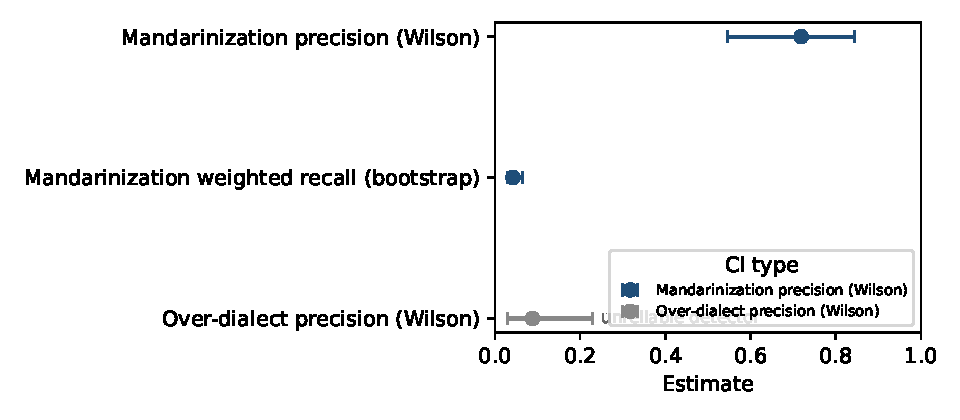
\includegraphics[width=\linewidth]{figures/audit_precision_recall.pdf}
\caption{Mandarinization precision and sampling-weighted recall.}
\label{fig:audit}
\end{figure}

\todo{precise but narrow: precision \MandPrec{} Wilson \MandPrecCI; weighted recall \MandRecallW{} bootstrap \MandRecallWCI}
\todo{over-dialect unreliable}
\todo{low-confidence controls \LowconfK/\LowconfN{} (mostly homophone/other)}
\todo{qualitative examples via \zh{}; pick from audit\_findings.md}

% PLACEHOLDER — outline only; no results prose yet
% target words: 500
\section{Discussion}
\todo{automatic mandarinization counts are a lower bound given recall \MandRecallW}
\todo{unadjusted vs adjusted filter signs as confounding, not a sign error; \HolmClause}
\todo{do not treat the over-dialect detector as a scientific result}

% PLACEHOLDER — outline only; no results prose yet
% target words: 350
\section{Limitations}
\begin{itemize}
\item \todo{Qwen3-ASR Sichuanese support and possible WSC-Eval leakage into its training data}
\item \todo{Whisper S1 and the LLM-GER merge were deferred, so P0 approximates the pipeline}
\item \todo{the over-dialect detector is unreliable}
\item \todo{a single annotator; intra-annotator $\kappa$ pending after a multi-week gap on reannotate\_ids.txt}
\item \todo{the lexicon was not retuned, so recall is lexicon-specific}
\item \todo{WVMOS / signal quality was not controlled}
\end{itemize}

% PLACEHOLDER — outline only; no results prose yet
% target words: 300
\section{Ethical considerations}
\todo{speaker and creator rights: audio not redistributed; IDs and labels only}
\todo{dialect speakers and representational harm from filtering}
\todo{the annotator is the author (a native-speaker bias note)}
\todo{dataset licence: verify WSC licence}
\todo{no personal data processed}

% PLACEHOLDER — outline only; no results prose yet
% target words: 150
\section{Conclusion}
\todo{restate the three RQs with macros only}
\todo{mandarinization detector precise but narrow; over-dialect unreliable}
\todo{filter: \FilterPassWord{} often unadjusted, OR \ORcmp, \HolmClause}


\bibliographystyle{acl_natbib}
\bibliography{refs}

\end{document}
